\label{sec:overview}

In this section, we introduce the background knowledge of false sharing 
%of cache lines in the memory hierarchy 
and motivate the necessity of a lightweight detection in multithreaded programs.

\subsection{Background of False Sharing}
\label{sec:background}

In the multicore era, multithreading is the basic way to utilize underlying hardware cores by running different threads on different cores concurrently. When a thread modifies data of a cache line, the underlying cache coherence protocol (inside hardware) silently invalidates the duplicates of this cache line on other cores. This is to guarantee correct executions for true sharing instances like that shown in Figure~\ref{fig:tsinfs}. However, for false sharing cases (e.g. Figure~\ref{fig:fsinfs}), these invalidations are totally unnecessary when different threads are actually accessing different parts of the same line. Cache invalidations may force other cores to wait for reloading of data unnecessarily, wasting CPU time and precious memory bandwidth. A big amount of unnecessary cache invalidations can significantly impact the performance of software. As shown by the example shown in Figure~\ref{fig:penalty}, the false sharing problems can slowdown the performance of applications as much as an order of magnitude. The hardware trend, including adding more cores into the same machine, introducing the Non-Uniform-Memory-Access (NUMA) architecture, or increasing the size of a cache line, will further degrade the performance of false sharing problems, making the task of detecting more urgent. 
%Actually, as the evolution of the hardware, such as the uses of larger cache lines or the popularity of Non-Uniform-Memory-Access hardware, the false sharing problem can become increasingly serious. 

The performance of false sharing can be avoidable because of unnecessary cache invalidations, while true sharing can not. False sharing can be further categorized into inter-object and intra-object false sharing. When two different objects in the same cache line are accessed by different threads simultaneously, that is inter-object false sharing. Otherwise, it is intra-object false sharing.  %Thus, it is urgent to develop some tools and systems to tackle with this problem. 

\begin{figure}[htbp]
\centering
\subfigure[False sharing]{%
   \label{fig:fsinfs}
   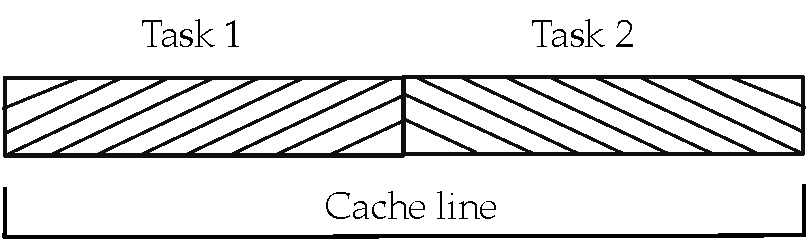
\includegraphics[width=2.4in]{figure/falsesharing}
}%
\hspace{30pt}
\subfigure[True sharing]{%
   \label{fig:tsinfs}
   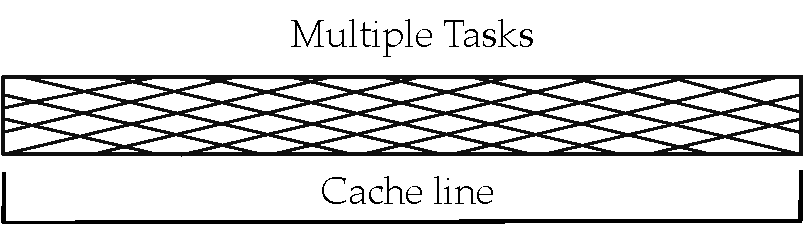
\includegraphics[width=2.4in]{figure/truesharing}
}%
\caption{False sharing (a) vs. true sharing (b). For false sharing, different tasks access different parts of the same cache line simultaneously. For true sharing, multiple tasks access the same part of a cache line.\label{fig:falsesharing}}
\end{figure}

Common programming practice can easily introduce false sharing. For an example shown in Figure~\ref{fig:penaltycode}, different threads access different words of the same global array, but involving in a big number of unnecessary cache invalidations. This problem is hard to find out manually by checking the results of executions.  

After the detection, there are several ways to fix them by preventing multiple threads from accessing the same cache line simultaneously. {\tt First},  we can pad useless words into a corresponding structure or class. {\tt Second}, we can assign the value of falsely-shared variable to a thread-local variable so that different threads may update their local variables, and commit those changes back to the shared variable in the end. {\tt Third},  some systems can isolate the execution of different threads, but with their own limitations on applications and the environment~\cite{sheriff, OSdetection}. 
%However, Sheriff only works for multithreaded programs that are using the standard \pthreads{} library, without ad hoc synchronizations~\cite{Xiong:2010:AHS:1924943.1924955} and communication across the stack. 
Thus, mostly people are still using the first two approaches to fix false sharing problems by changing the code manually. For these approaches, programmers should have precise information about falsely-shared objects in order to fix them. \cheetah{} aims to provide precise information as much as possible, such as where are those falsely-shared objects, what is access pattern of memory accesses, and how much performance improvement after fixes. 


\sloppy
\subsection{Motivation of Efficient Memory Trace Collection}
Analyzing memory access patterns is an effective method to pinpoint false sharing. However, capturing memory accesses of software is costly, even with various sampling techniques~\cite{}. The overhead can as high as 2-5$\times$, which is often not applicable to real applications working on large data sets and running in a highly threaded platform. 

To address this issue, recent hardware performance monitoring units (PMU) support sampling memory accesses with extremely low overhead, less than 5\%. There are two typical sampling mechanisms in modern architectures: instruction-based sampling (IBS)~\cite{} supported in AMD Opteron processors and precise event-based sampling (PEBS)~\cite{} in Intel Sandy Bridge processors as well as their successors. Both IBS and PEBS can sparsely sample memory loads and stores at the same time. For each load sample, IBS and PEBS capture its effective address and the latency in cycles for fetching the data. For each store sample, IBS and PEBS capture its effective address only. Moreover, both IBS and PEBS record the precise instruction pointers of sampled memory accesses, which can be used to associate the analysis with program's source code. To make our analysis efficient, we build our tool based on PMU sampling. 


\section{Detecting False Sharing}
\label{sec:basicidea}
% What is the basic idea? Why those ones uses performance counters can not reveal false sharing problems? 
\cheetah{} aims to report false sharing problems having significant performance impact, where a large number of cache invalidations occur on those cache lines. However, it is not easy to know whether a cache line is invalidated or not, without the complete information of cache hierarchy and different threads' running situation. 

\cheetah{} avoids these information and computes the number of cache invalidations according to a basic rule: {\it \bf if a thread writes a cache line after other threads have accessed the same cache line, this write operation causes a cache invalidation}. To make it true, \cheetah{} further makes the following \textbf{two basic assumptions}.

\begin{itemize} 
\item {\bf Assumption 1:} Each thread runs on a separate core with its own cache. 

\item {\bf Assumption 2: } The sizes of caches are infinite. 
 
\end{itemize}

Assumption 1 is a reasonable assumption since different threads can run on a separate core, even if they may not in a given execution. If multiple threads are actually running on the same core, false sharing problems may cause less performance penalty. In this meaning, assumption 1 actually presents the worst scenario for a given false sharing. This assumption provides the following benefits: there is no need to know the actual situation where a thread is running by assuming different threads are running on different cores; there is no need to know actual cache hierarchy by assuming different cores having their own cache (at least L1). 

Assumption 2 further assumes that the sizes of caches are infinite. If there is a memory access within a cache line, the hardware cache (of running this thread) always holds the data until an access of other threads (running on other cores by assumption 1) invalidates it. Thus, there is no need to track cache evictions that are caused by cache capacity. 

Combining with these two assumptions, \cheetah{} can practically compute the number of cache validations simply by checking the pattern of memory accesses without knowing the actual running condition of different threads or cache hierarchy: if a memory access of a thread will load this cache line on its own cache (assumption 1), then only a write from a different thread can invalidate this cache line. Thus, we can report the number of cache validations by only observing the memory access pattern, similar to previous work~\cite{Predator, qinzhao}. 
%This idea is very similar to Predator~\cite{Predator}. \Cheetah{} will rely on hardware-performance counters to reduce performance overhead of detection, instead of a instrumentation-based approach~\cite{Predator}. 

 
% This idea is similar to Predator. But Predator is a compiler-based approach, which needs to change the source code of applications. Also, it introduces much performance overhead that can block its use in deployment environment. 

% To reduce the performance overhead, 
% Basic idea, by examing the memory access pattern

\subsection{Sampling Memory Accesses}
\label{sec:perfcounter}

According to the basic rule described above, it is very important to track memory accesses of different threads in order to compute the number of cache invalidations on each cache line. 

The previous work \Predator{} leverages on compiler instrumentation to insert function calls before every memory access that is going to handled by \Predator{}'s runtime system~\cite{Predator}. However, this approach introduces more than $5\times$ performance overhead by instrumenting every memory access. More than that, \Predator{} has to re-compile applications, which needs the availability of source code. \Predator{} is not desirable for legacy applications without the source code, or real deployment that is sensitive to performance. 

\cheetah{} aims to significantly reduce the performance overhead by leveraging hardware performance counters that are available on most modern hardware. Hardware performance counters provide sampling-based memory access information about how the hardware is being exercised by a program, such as read/write operations, memory addresses, and threads~\cite{Mucci99papi}. These information is enough to compute the number of cache invalidations based on the basic rule that is described in Section~\ref{sec:basicidea}. Since hardware performance counter only samples a memory access out of a specified number, it doesn't pose significant performance overhead. 
Besides that, using performance counters does not need to instrument source code explicitly, thus providing a non-intrusive way to monitor memory references. 

\cheetah{} is different with existing approaches using hardware performance counters to detect false sharing problems~\cite{mldetect, openmp, detect:ptu}. Jayasena et. al. collects different types of events like memory accesses, data caches, TLBs, interactions among cores, and resources stalls, and derives potential memory patterns that can cause false sharing~\cite{mldetect}. DARWIN collects cache coherence events at the first round, then identifies possible memory accesses on those data structures that are involved in frequent cache invalidations for the second round~\cite{openmp}. DARWIN also requires manual effort or expertise to verify whether false sharing occurs or not.  Intel's PTU also relies on memory sampling mechanism but can not differentiate false sharing and true sharing since it discards the temporal information of memory accesses~\cite{detect:ptu}. More details on the difference have been discussed in Section~\ref{sec:relatedwork}.

\subsection{Computing Cache Invalidations}
\label{sec:computeinvalidations}

\Cheetah{} targets to report false sharing that can have performance impact on applications. \Cheetah{} focuses on those false sharing problems with a significant number of cache invalidations.  

Qin Zhao et. al. propose to compute the number of cache invalidations based on the ownership of cache lines: when a thread updates an object that it does not own, it will cause cache invalidations and set the owner to the current thread~\cite{qinzhao}. However, this approach cannot be easily to scalable to more than 32 threads because of excessive memory consumption, where every word with 32-bits can only tracking 32 threads. Also it introduce significant performance overhead by utilizing the dynamic instrumentation technique and maintaining ownership of different cache lines. 

To overcome these shortcomings, \Cheetah{} maintains a two-entries-table ($T$) for each cache line ($L$) that is borrowed from Predator~\cite{Predator}, where each entry tracks accesses from one thread in a period. \Cheetah{} also keeps a counter for every cache line that indicates the number of cache invalidations on this cache line.  
According to the basic rule that are described in Section~\ref{sec:basicidea}, only a write access can cause a cache invalidation. When there is a cache invalidation, the current write access will flush the table and will be added into its corresponding table ($T$). Thus, a table will always have an entry except in the beginning. More specifically, \cheetah{} checks possible cache invalidations as follows.
 
\begin{itemize}
\item
  For each read access $R$, \cheetah{} will check: 
  \begin{itemize}
    \item
      If $T$ is full, there is no need to record this read access.
    \item
      If $T$ is not full and the existing entry has a different thread ID, 
      then \cheetah{} records this read access by adding a new entry to the table.
  \end{itemize}
\item
  For each write access $W$,  
  \begin{itemize}
    \item
      If $T$ is full, then $W$ causes a cache invalidation since at least one of two existing entries are issued by another thread (on another core).
    \item
      If $T$ is not full (and not empty),
      \cheetah{} checks whether the current $W$ is from the same thread as the existing entry . If
      so, $W$ will not cause a cache invalidation. Otherwise, there is a cache invalidation caused by this $W$.
  \end{itemize}
\end{itemize}

      
In the end, 
\cheetah{} can collect the number of cache invalidations happened on each cache line.  


\subsection{Shadow Memory and Custom Heap}

For each sampled memory access, \cheetah{} has to locate a specific cache line and compute the cache invalidations. \Cheetah{} utilizes the shadow memory mechanism to speedup the locating process. Shadow memory has been utilized extensively in different fields, such as detecting concurrency bugs~\cite{Harrow:2000:RCM:645880.672080, helgrind, 404681, Savage:1997:EDD:268998.266641}, tracking information flow or data flow~\cite{Cheng:2006:TEF:1157733.1157903, Newsome05dynamictaint, Qin:2006:LLP:1194816.1194834}, or detecting memory errors or others~\cite{qinzhao, Hastings91purify:fast, Seward:2005:UVD:1247360.1247362, Narayanasamy:2006:ALO:1140277.1140303}. 

It is very hard to know the range of heap memory if using the default heap, which complicates the implementation of the shadow memory mechanism. Thus, \cheetah{} built its custom heap based on Heap Layers~\cite{Berger:2001:CHM:378795.378821}. \cheetah{} pre-allocates a fixed size of memory
from its underlying operating system using \texttt{mmap} system calls and satisfies memory allocations from this block of memory. \cheetah{} also adapts the per-thread heap organization used by Hoard~\cite{Hoard}. 

Each heap object has the size of {\it power of $2$}, known as block size. When an object is allocated, \cheetah{} adds an object header to each object, which has the size information of each object. To find out where an heap is allocated, \cheetah{} also stores its allocation call stack on its header, thus it can report the line information of falsely-shared objects. 

However, by utilizing its custom heap, \cheetah{} can not report false sharing problems caused by the heap allocator. For example, some heap allocators may allocate two objects in the same cache line to two different threads, which can also cause false sharing problems. But we argue that this problem should be fixed by using a modern heap allocator like Hoard~\cite{Hoard}.  
%\cheetah{} only reports those false sharing problems that can have a significant impact on the performance by predicting the upper bound of performance improvement, according to the idea that are discussed in Section~\ref{sec:predictidea}.  It will rank the severity of performance degradation of any detected false sharing problems based on the predicted performance improvement after fixes.

\section{Assessing Performance Impact}
\label{sec:predictidea}

\paragraph{Current problem:} None of existing tools can assess the performance impact of false sharing instances~\cite{sheriff, Predator, openmp}. At most, they can report the number of cache invalidations caused by a particular false sharing problem. Unfortunately, the number of cache invalidations does not equal to the potential performance impact after fixing, where fixing a falsely-shared program with a big number of cache invalidations may not improve its performance. Thus, existing tools reported some insignificant false sharing problems. For example, fixing reported false sharing in reverse\_index brings less than 1\% performance improvement~\cite{sheriff, Predator}. Insignificant false sharing instances are not false positives, but reporting them increases manual burden for programmers, without performance benefit. 

Different with all existing tools, \Cheetah{} only reports false sharing problems that will have significant performance impact after fixes. \Cheetah{} utilizes the latency information (e.g. cycles) of every memory access that can be provided by performance monitoring units, either Intel's PEBS registers or AMD's IBS registers, to assess the performance impact of false sharing problems. 

\Cheetah{} first assumes that the sampling results represent the whole execution, which is reasonable given that sampling is evenly distributed among the whole execution. Since performance monitoring units can only provide the latency information of cycles, \Cheetah{} uses the sum of cycles to represent the running time in the assessment.  

{\bf The basic idea of prediction is to compute the performance improvement if the actual cycles of every memory access on a
falsely-shared object are replaced by the average cycles of every memory access without false sharing}. Since fixing one false sharing may affect the latency on other memory addresses, \cheetah{} further assumes that the latency of other memory accesses are intact. \cheetah{} will compute the performance improvement based on EQ.(\ref{eq:improvement}), where runtime is denoted by $RT$. 
\begin{equation}
\label{eq:improvement}
Perf_{improve}=RT_{actual}/RT_{predict}
\end{equation} 


In reality, \Cheetah{} presents a upper bound on the performance improvement percentage, but not an absolute value of time saving. 
%For example, padding unnecessary words into structures or classes (as described in Section~\ref{sec:background}) can reduce the memory efficiency and may even degrade the performance of an application~\cite{qinzhao}. 
Detailed algorithms to compute $RT_{actual}$ and $RT_{predict}$ are detailed in Section~\ref{sec:predictimprove}. We also evaluate the precision of our prediction in Section~\ref{sec:evalperfpred}.


